\chapter{Ranked Retrieval}
\begin{multicols*}{2}

\noindent Boolean queries are not suitable for most users and often results in either too few or too many results. In ranked retrieval, users can use natural language for query and we only show top 10 results. \\

\noindent In bag-of-words model, vector representation doesn’t consider the ordering of word in a document.\\

\noindent Term frequency is the number of times a term occurs in a document. \\

$$w_{t,d} = 
\begin{cases}
    1 + log_{10} \text{tf}_{t,d} & \text{tf}_{t,d} > 0 \\
    0 & \text{otherwise}
\end{cases}
$$

\noindent Document frequency is number of times a term occurs in a collection of documents. Rare term has low document frequency, and is more informative than frequent terms. Inverse document frequency has no effect on one-term queries.

$$\text{idf}_t = log_{10} \frac{N}{\text{df}_t}$$

\noindent TF-IDF weighting: 

$$w_{t,d} = (1+ log_{10} \text{tf}_{t,d})\times log_{10} \frac{N}{\text{df}_t}$$

\noindent SMART Notation: \verb|ddd.qqq|
\begin{center}
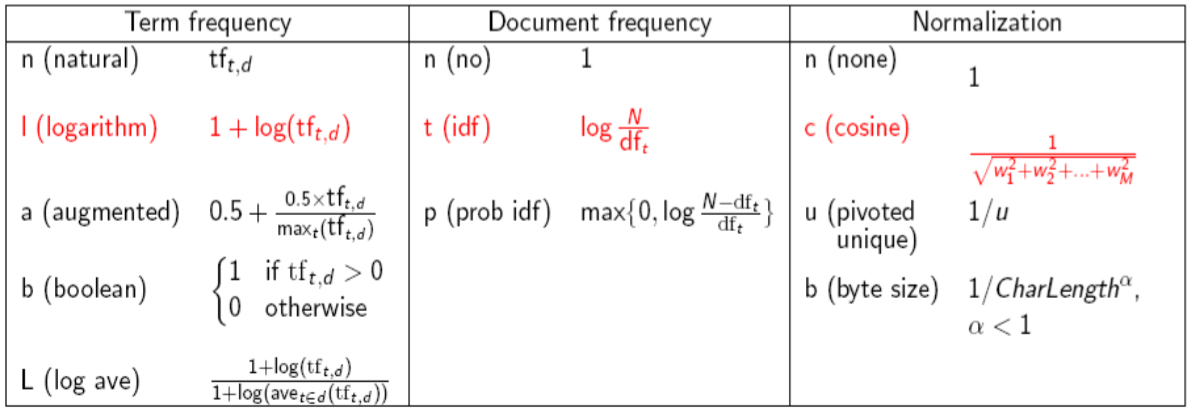
\includegraphics[width=8cm]{smart-notion}
\end{center}

\noindent Example: \verb|lnc.ltc|
\begin{center}
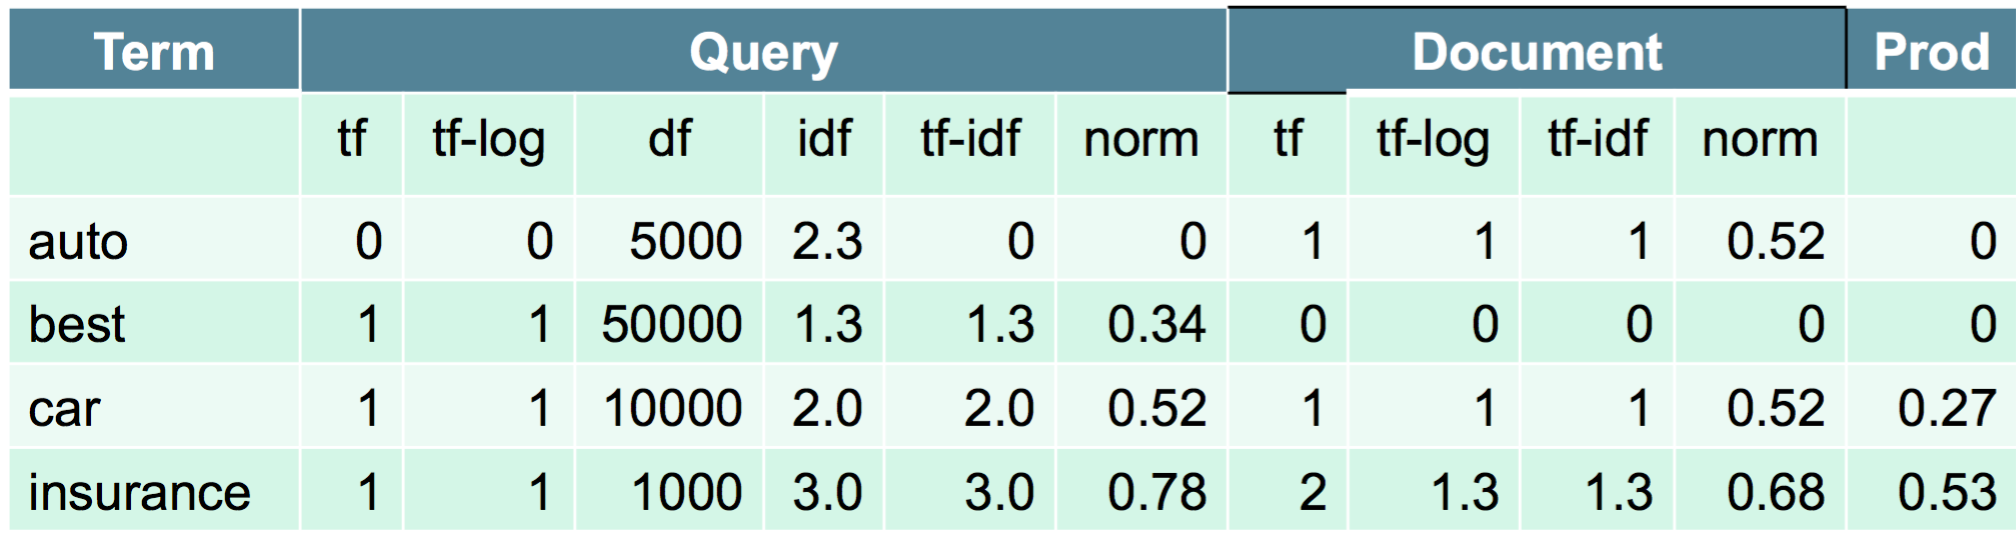
\includegraphics[width=8cm]{smart-notion-example}
\end{center}

\noindent We rank documents according to their proximity to the query in vector space. Proximity can be measured using Euclidean Distance or Cosine Similarity.

$$\text{dist}(A,B) = \sqrt{(x_A - x_B)^2 + (y_A - y_B)^2}$$

$$\text{cosine} (\vec{q},\vec{d}) = \frac{\vec{q} \cdot \vec{d}}{|\vec{q}||\vec{d}|}$$

\end{multicols*}
